\documentclass[tikz]{standalone}

\begin{document}

\tikzset{every picture/.style={line width=0.75pt}} %set default line width to 0.75pt        

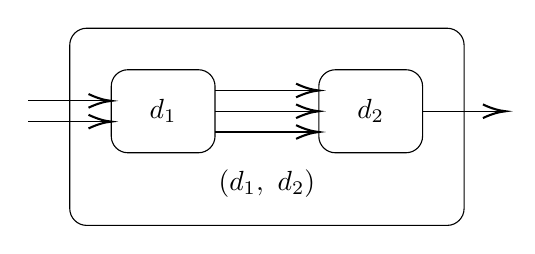
\begin{tikzpicture}[x=0.75pt,y=0.75pt,yscale=-1,xscale=1]
  %uncomment if require: \path (0,150); %set diagram left start at 0, and has height of 150

  %Rounded Rect [id:dp7037699547873038] 
  \draw (150,38) .. controls (150,33.58) and (153.58,30) .. (158,30) -- (192,30) .. controls (196.42,30) and
  (200,33.58) .. (200,38) -- (200,62) .. controls (200,66.42) and (196.42,70) .. (192,70) -- (158,70) .. controls
  (153.58,70) and (150,66.42) .. (150,62) -- cycle ;
  %Rounded Rect [id:dp30618805023006357] 
  \draw (50,38) .. controls (50,33.58) and (53.58,30) .. (58,30) -- (92,30) .. controls (96.42,30) and (100,33.58) ..
  (100,38) -- (100,62) .. controls (100,66.42) and (96.42,70) .. (92,70) -- (58,70) .. controls (53.58,70) and
  (50,66.42)
  .. (50,62) -- cycle ;
  %Rounded Rect [id:dp45117241599728874] 
  \draw (30,18.18) .. controls (30,13.66) and (33.66,10) .. (38.18,10) -- (211.82,10) .. controls (216.34,10) and
  (220,13.66) .. (220,18.18) -- (220,96.82) .. controls (220,101.34) and (216.34,105) .. (211.82,105) -- (38.18,105) ..
  controls (33.66,105) and (30,101.34) .. (30,96.82) -- cycle ;
  %Straight Lines [id:da9955123946130728] 
  \draw  (10,55) -- (48,55) ;
  \draw [shift={(50,55)}, rotate = 180] [color={rgb, 255:red, 0; green, 0; blue, 0 }  ][line width=0.75]
  (10.93,-3.29)
  .. controls (6.95,-1.4) and (3.31,-0.3) .. (0,0) .. controls (3.31,0.3) and (6.95,1.4) .. (10.93,3.29)	 ;
  %Straight Lines [id:da418746828285135] 
  \draw  (200,50) -- (238,50) ;
  \draw [shift={(240,50)}, rotate = 180] [color={rgb, 255:red, 0; green, 0; blue, 0 }  ][line width=0.75]
  (10.93,-3.29) .. controls (6.95,-1.4) and (3.31,-0.3) .. (0,0) .. controls (3.31,0.3) and (6.95,1.4) .. (10.93,3.29)
  ;
  %Straight Lines [id:da4282424423950084] 
  \draw  (10,45) -- (48,45) ;
  \draw [shift={(50,45)}, rotate = 180] [color={rgb, 255:red, 0; green, 0; blue, 0 }  ][line width=0.75]
  (10.93,-3.29)
  .. controls (6.95,-1.4) and (3.31,-0.3) .. (0,0) .. controls (3.31,0.3) and (6.95,1.4) .. (10.93,3.29)	 ;
  %Straight Lines [id:da6971913985972173] 
  \draw  (100,40) -- (148,40) ;
  \draw [shift={(150,40)}, rotate = 180] [color={rgb, 255:red, 0; green, 0; blue, 0 }  ][line width=0.75]
  (10.93,-3.29) .. controls (6.95,-1.4) and (3.31,-0.3) .. (0,0) .. controls (3.31,0.3) and (6.95,1.4) .. (10.93,3.29)
  ;
  %Straight Lines [id:da1593358832118874] 
  \draw  (100,50) -- (148,50) ;
  \draw [shift={(150,50)}, rotate = 180] [color={rgb, 255:red, 0; green, 0; blue, 0 }  ][line width=0.75]
  (10.93,-3.29) .. controls (6.95,-1.4) and (3.31,-0.3) .. (0,0) .. controls (3.31,0.3) and (6.95,1.4) .. (10.93,3.29)
  ;
  %Straight Lines [id:da9265626009713097] 
  \draw  (100,60) -- (148,60) ;
  \draw [shift={(150,60)}, rotate = 180] [color={rgb, 255:red, 0; green, 0; blue, 0 }  ][line width=0.75]
  (10.93,-3.29) .. controls (6.95,-1.4) and (3.31,-0.3) .. (0,0) .. controls (3.31,0.3) and (6.95,1.4) .. (10.93,3.29)
  ;

  % Text Node
  \draw (125,85) node	[align=left] {$\displaystyle \Sequential( d_{1} ,\ d_{2})$};
  % Text Node
  \draw (75,50) node   [align=left] {$\displaystyle d_{1}$};
  % Text Node
  \draw (175,50) node	[align=left] {$\displaystyle d_{2}$};

\end{tikzpicture}
\end{document}
